\section{Android}


\subsection{ADB}
It really makes a lot of sense to use a physical phone instead of an emulated one. To be able to communicate with your phone, however, you need the adb-server to be aware of the phone. There is a commandline-tool, \verb adb, that you can use to have the adb-server talk to your phone. However, to be able to do that, you must first set up your phone accordingly. 
\begin{itemize}
    \item on your linux-machine, install \verb mtp-tools and \verb mtpfs . 
    \item mount your phone using a \emph{data} usb-cable
    \item enable developer-mode 
    \item have your phone use the MTP protocol
\end{itemize}
With that given, you should be able to see your phone with \inlinecode{lsusb} and \inlinecode{adb devices}.

\subsection{Basic concepts}

\paragraph{The structure of an app} is as follows: the compiled java-bytecode\footnote{actually, your code gets compiled to java-bytecode (i.e. several \verb .class files), but from there is is compiled on to a single \verb .DEX file to be run on androids version of the JRE, the ART.}, togehter with all libraries and resources, is packaged into an APK (android application package), analog to a jar or a war. 

\paragraph{The mainfest} mostly tells the phone some meta-info about the APK; like what rights are required, what SDK version is required, what the main-activity is, and such. 

\paragraph{A layout} describes the app's appearence on one screen. Written in XML. The layout can be found in \verb res/layout. Within a layout file, you can reference data from \verb res/values/strings.xml by using the string \verb "@string/app\_someStringName" .

\paragraph{An activity} is a single, defined thing that your user can do. Activities are usually associated with one screen. In code, an activity is represented by a single class extending the class \inlinecode{Activity}. It largely has the role of \emph{controller}, negotiating between the \emph{view.xml} and a custom-class-backend. All activities need to be declared in the manifest.

\paragraph{An intent} is a type of message that one activity can send to another. It can be used to start another activity within the same app or even in another app. It can even be broadcasted to all apps on the phone so that any app that might be able to handle the request may use it. 
Here is an example of how we might use an intent to switch to another activity: 
\begin{lstlisting}[language=java]
letsGoButton = (Button) findViewById(R.id.startGameButton);
letsGoButton.setOnClickListener(new View.OnClickListener() {
	public void onClick(View view) {
		Intent goToGameActivity = new Intent(MainActivity.this, PlayActivity.class);
		startActivity(goToGameActivity);
	}
});
\end{lstlisting}


\paragraph{A view} is a custom drawable thing, like buttons or menus. You create such a view when the predefined UI-elements don't suite your needs, like when you want to create an animation. You create a view by extending \inlinecode{View} and implementing \inlinecode{onDraw(Canvas canvas), onTouchEvent(MotionEvent event)}, etc.

\paragraph{The file R.java} is an automatically created file that android uses to keep track of the resources available to your app. For example, your activity will tell the phone to use the \verb activity_play.xml layout file by going \inlinecode{setContentView(R.layout.activity_play);} inside the \verb onCreate method. We can access things in \verb R very much like we can in the \verb DOM .




\subsection{Userinput}
Android apps behave very much like html forms. 

The steps are: 
\begin{itemize}
    \item The main-activity choses a layout (in this case, \inlinecode{activity_find_beer.xml}) that is to be displayed by using 
    \begin{lstlisting}
        protected void onCreate(Bundle savedInstanceState) {
            super.onCreate(savedInstanceState);
            setContentView(R.layout.activity_find_beer);
        }
    \end{lstlisting}
    
    \item The layout specifies which method to call in the activity when a button is pressed. A button can have an attribute \inlinecode{android:onClick:"onClickFindBeer"}
    
    \item A click now is passed trhough to the activity, calling the method \inlinecode{public void onClickFindBeer(View view) }. In this case, \inlinecode{view} refers to the button that was pressed. 
    
    \item Anywhere in the application logic, the activity can get a hold of any element of the layout by using \inlinecode{findViewById()} like this: 
    \begin{lstlisting}
    TextView brands = (TextView) findViewById(R.id.brands);
    brands.setText("Gottle of geer");
    \end{lstlisting}
\end{itemize}




\subsection{Activities}
This section handles activities in more detail. 
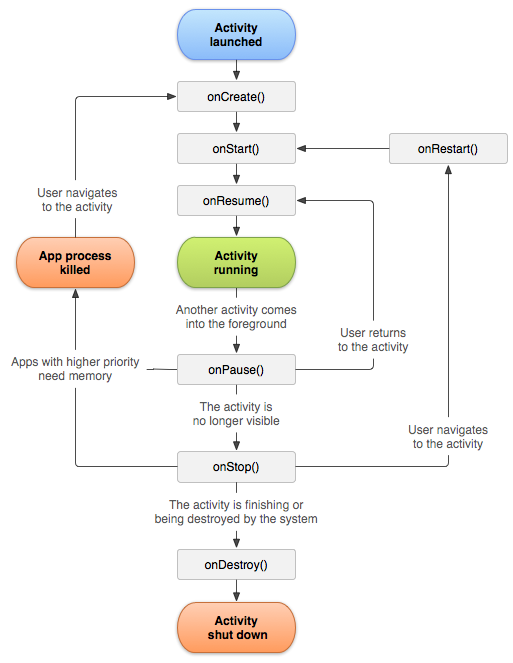
\includegraphics[scale=0.4]{images/activity_lifecycle.png}





\subsection{Threading}

\paragraph{Threads} come in three different flavors:

\begin{itemize}
    \item the main thread (aka. ui-thread)
        \begin{itemize}
            \item listens for intents
            \item listens for input (touch/speak) events
        \end{itemize}
    
    \item the render thread
        \begin{itemize}
            \item You don't normally interact with that thread. The main-thread passes it views to render, and the render thread executes the views \inlinecode{onDraw} methods. 
            \item However, you can steal work from it by creating a special kind of view: a \inlinecode{SurfaceView}. This kind of view exposes a canvas that is to be rendered in a custom thread.  
        \end{itemize}
        
    \item custom threads
        \begin{itemize}
            \item simple custom threads extending \inlinecode{Thread}
            \item android-specific custom threads extending \inlinecode{AsyncTask}
        \end{itemize}
\end{itemize}

\paragraph{Handlers} are a different thing than threads. They are not separate theads, they just postpone the execution of code. There basically promises: some code will be executed asynchronously, but sitll on the main thread. There are two usecases for handlers: 

\begin{itemize}
    \item You really want an action to happen on the main-thread, but at a later time. For example, ....
    \item Custom threads are not allowed to manipulate UI-elements on the main-thread. Instead, pass them a handler from the main-thread so they can call the handler. In other words: handlers are a (android-specific) method of inter-thread communication. 
\end{itemize}


\subsection{Drawing}
There are three ways of drawing in android apps. 
\begin{itemize}
    \item When you only need a single animated item in an overal static UI, draw your animations into a view.
    \item When you want your drawing to be updated regularly, use a canvas. 
    \item When you want to do 3d-rendering, use the OpenGL-API.
\end{itemize}


\paragraph{Using a custom view} is certainly the most straightforward way of creating graphics. Consider this simple example: 

\begin{lstlisting}[language=java]
public class PlayActivity extends AppCompatActivity {

    @Override
    protected void onCreate(Bundle savedInstanceState) {
        super.onCreate(savedInstanceState);
        setContentView(new FullScreenView(this));
    }
}
\end{lstlisting}

\begin{lstlisting}[language=java]
public class FullScreenView extends View {

    private Rect lilRect;
    private Paint painter;
    private static final int SQUARE_SIDE_LENGTH = 200;

    public FullScreenView(Context context) {
        super(context);
        lilRect = new Rect(30, 30, SQUARE_SIDE_LENGTH, SQUARE_SIDE_LENGTH);
        painter = new Paint();
        painter.setColor(Color.MAGENTA);
    }

    @Override
    protected void onDraw(Canvas canvas) {
        canvas.drawRGB(39, 111, 184);
        canvas.drawRect(lilRect, painter);
    }

    @Override
    public boolean onTouchEvent(MotionEvent event) {
        lilRect.left = (int) (event.getX() - (SQUARE_SIDE_LENGTH / 2));
        lilRect.right = (int) (event.getX() + (SQUARE_SIDE_LENGTH / 2));
        lilRect.top = (int) (event.getY() - (SQUARE_SIDE_LENGTH / 2));
        lilRect.bottom = (int) (event.getY() + (SQUARE_SIDE_LENGTH / 2));
        invalidate();
        return true;
    }
}
\end{lstlisting}


\paragraph{Using the canvas} is a lot more direct than using a view-object. We still make use of a custom view, but instead of calling \inlinecode{invalidate()} when we're ready to draw, we host the game-loop inside the view and act upon the canvas directly. 

\begin{lstlisting}
public class MainActivity extends AppCompatActivity {

    @Override
    protected void onCreate(Bundle savedInstanceState) {
        super.onCreate(savedInstanceState);
        SceneLogic boardScene = new BoardScene();
        MainView mainView = new MainView(this, boardScene);
        setContentView(mainView);
        mainView.startRenderThread();
    }
}
\end{lstlisting}

\begin{lstlisting}
/**
 * This class is there to present the SurfaceHolder as well as any touch- or system-events
 * to the RenderThread.
 */
public class MainView extends SurfaceView implements SurfaceHolder.Callback {

    private RenderThread renderThread;

    public MainView(Context context, SceneLogic sceneLogic) {
        super(context);
        SurfaceHolder surfaceHolder = getHolder();
        surfaceHolder.addCallback(this);
        renderThread = new RenderThread(context, surfaceHolder, sceneLogic);
    }

    public void startRenderThread() {
        renderThread.start();
    }

    public void stopRenderThread() {
        renderThread.setInactive();
    }

    @Override
    public boolean onTouchEvent(MotionEvent event) {
        return renderThread.getLogic().onTouch(event);
    }

    @Override
    public void surfaceCreated(SurfaceHolder surfaceHolder) {}

    @Override
    public void surfaceChanged(SurfaceHolder surfaceHolder, int i, int i1, int i2) {}

    @Override
    public void surfaceDestroyed(SurfaceHolder surfaceHolder) {}

}
\end{lstlisting}


\begin{lstlisting}
public class RenderThread extends Thread {

    private final long frameTime = 17;   // How long (in millisec) a frame may take
    private SceneLogic sceneLogic;
    private Context context;
    private SurfaceHolder surfaceHolder;
    private boolean running;

    public RenderThread(Context context, SurfaceHolder surfaceHolder, SceneLogic sceneLogic) {
        this.context = context;
        this.surfaceHolder = surfaceHolder;
        this.running = true;
        this.sceneLogic = sceneLogic;
    }

    @Override
    public void run() {
        long updateDuration = 0;
        long sleepDuration = 0;

        while(running) {

            // Step 0 : how long did the loop take?
            long beforeUpdateRender = System.nanoTime();
            long delta = sleepDuration + updateDuration;

            // Step 1 : scene logic
            sceneLogic.update(delta);

            // Step 2: scene rendering
            Canvas canvas = surfaceHolder.lockCanvas();
            if(canvas != null) {
                sceneLogic.draw(canvas);
                surfaceHolder.unlockCanvasAndPost(canvas);
            }

            // Step 3: sleep for remainder of frameTime
            updateDuration = (System.nanoTime() - beforeUpdateRender) / 1000000L;
            sleepDuration = Math.max(2, frameTime - updateDuration);
            try{
                Thread.sleep(sleepDuration);
            } catch (Exception e) {
                e.printStackTrace();
            }


        }
    }

    public SceneLogic getLogic() {
        return sceneLogic;
    }

    public void setInactive() {
        running = false;
    }
}
\end{lstlisting}










\section{VR on android}

\subsection{Basic app} 

\paragraph{The manifest} should basically be a variant of this: 
\begin{lstlisting}[language=xml]
<manifest ...
    <uses-permission android:name="android.permission.READ_EXTERNAL_STORAGE" />
    ...
    <uses-sdk android:minSdkVersion="19" android:targetSdkVersion="24"/>
    ...
    <uses-feature android:glEsVersion="0x00020000" android:required="true" />
    <uses-feature android:name="android.software.vr.mode" android:required="false"/>
    <uses-feature android:name="android.hardware.vr.high_performance" android:required="false"/>
    ...
    <application
            android:theme="@style/VrActivityTheme"
            ...
        <activity
                android:name=".TreasureHuntActivity
                ...
                android:screenOrientation="landscape"
                android:configChanges="orientation|keyboardHidden|screenSize|uiMode|navigation"
                android:enableVrMode="@string/gvr_vr_mode_component"
                android:resizeableActivity="false">
                ...

            <intent-filter>
                <action android:name="android.intent.action.MAIN" />
                <category android:name="android.intent.category.LAUNCHER" />
                <category android:name="com.google.intent.category.CARDBOARD" />
                <category android:name="com.google.intent.category.DAYDREAM" />
            </intent-filter>
        </activity>
    </application>
</manifest>
\end{lstlisting}

\paragraph{Gradle} handles the specific dependencies that are required to make a 3d-app. At least you're going to need: 
\begin{lstlisting}
allprojects {
    repositories {
        jcenter() // this is where we get the vr libraries
    }
}
model {
    android {
        ...
        buildTypes {
            release {
                minifyEnabled true
                // Progueard minifies the APK. This line makes sure it doesn't obfuscate vr-libs.
                proguardFiles.add(file('../../proguard-gvr.txt'))
            }
        }
    }
}
dependencies {
    classpath 'com.android.tools.build:gradle:2.3.3'
    compile 'com.google.vr:sdk-base:1.120.0'
    compile 'com.google.vr:sdk-audio:1.120.0'
}
\end{lstlisting}

\paragraph{The layout} in a vr-app is very simple. There is only one element to use: the \verb com.google.vr.sdk.base.GvrView element.

\paragraph{The main task} should in most case extend \inlinecode{GvrActivity}. This way, your activity gets access to a load of VR events. 